Since the first approach failed to deliver reasonable results, no matter the network's configuration, one may rethink the fundamentals: the data itself. The topic of this work is about the term structures formed by the futures' prices. Therefore the inputs of the network need to represent this term structure in some way and consequently are not subject to large changes. The situation is different for the output. Even though targeting spread prices seems natural, restructuring the data is certainly viable.

In this chapter the networks only have a single output. Having to predict only one value simplifies the task itself. First, the newly arranged data is described in more detail, followed by a short description of the adjusted network architecture. By evaluating and comparing the results of different experiments this chapter is concluded.

\section{Data description}

The available data is the same as in chapter~\ref{ch:all-at-once}. Therefore the properties are generally the same. The goal is to rearrange the data to simplify the learning process for the network. 

There are two obvious alternatives for ordering the spread prices to get a one-dimensional target:

\begin{enumerate}
	\item As futures are issued per month they can be be represented in this manner, forming twelve vectors corresponding the the months of a year
	\item They can also be represented in a similar manner to the first approach: as legs of a term structure, hence forming six vectors
\end{enumerate}

This chapter explores the necessary transformations and properties of these representations while also describing possible adjustments of the input data.

\subsection{Monthly representation}
\label{sec:oao-monthly-representation}

Each future has a corresponding symbol, assigning it to its month of expiration. By calculating the long spread prices using \eqref{eq:long-spread} and assigning the results the same symbol as $m_i$ one can easily filter the spreads by month. This result in a total of 15,193 values.

Looking at table~\ref{tab:spreads-by-month} there are around 1,266 values available per month with mostly similar properties. These can be used for training twelve specialized networks using the term structure as input and targeting only the corresponding month's spread price. Another advantage besides simplification is the implicit inclusion of seasonality.

\begin{table}
	\centering
	\caption[Descriptive statistics for spread prices by month]{Descriptive statistics for spread prices by month as described in section~\ref{sec:oao-monthly-representation}. Notice the outliers for November and December which can again be attributed to the 2008 financial crisis.}
\begin{tabular}{lllllllll}
	\toprule
	{} &  Count &   Mean &  Std. &    Min. &   25\% &   50\% &   75\% &  Max. \\
	\midrule
	Jan &  1281 &   0.54 &  0.67 &   -3.06 &   0.15 &   0.40 &   0.87 &  2.75 \\
	Feb &  1239 &   0.25 &  0.61 &   -1.55 &   0.00 &   0.18 &   0.35 &  4.90 \\
	Mar &  1238 &  -0.06 &  0.58 &   -3.05 &  -0.23 &  -0.05 &   0.22 &  1.55 \\
	Apr &  1329 &   0.28 &  0.53 &   -2.89 &   0.05 &   0.22 &   0.45 &  3.60 \\
	May &  1289 &   0.04 &  0.56 &   -3.97 &  -0.10 &   0.07 &   0.21 &  2.75 \\
	Jun &  1279 &   0.03 &  0.39 &   -2.24 &  -0.15 &  -0.01 &   0.16 &  1.86 \\
	Jul &  1328 &   0.32 &  0.46 &   -2.72 &   0.10 &   0.28 &   0.47 &  3.12 \\
	Aug &  1224 &  -0.13 &  0.43 &   -2.03 &  -0.30 &  -0.10 &   0.05 &  2.85 \\
	Sep &  1236 &   0.29 &  0.67 &   -7.08 &   0.09 &   0.21 &   0.45 &  3.60 \\
	Oct &  1281 &   0.31 &  0.65 &   -4.01 &   0.10 &   0.23 &   0.45 &  3.30 \\
	Nov &  1256 &   0.23 &  0.93 &  -13.68 &   0.10 &   0.24 &   0.45 &  3.54 \\
	Dec &  1213 &  -0.87 &  1.15 &  -10.90 &  -0.94 &  -0.60 &  -0.33 &  1.64 \\
	\bottomrule
	\end{tabular}
	\label{tab:spreads-by-month}
\end{table}

\subsubsection{Adjusting the input structure}

Just using the same input representation as in the first approach -- the difference over the futures prices' term structure -- leads to bad performance. The reason might be that the above mentioned seasonality can not be learned with how the data is currently structured. With futures price $m_i$ and spread price $v_i$ (of the next day) the network learns some mapping:

\begin{equation}
	\begin{bmatrix}
	m_1 & \cdots & m_8
	\end{bmatrix}^\top
	\mapsto v \in \{v_2, \dots, v_7\}
\end{equation}

On the one hand it is assured that target $v$ is the spread price of a certain month. However, there is no information about the spread's term structure included. (is it $v = v_1$ or $v = v_2$ or\dots?) On the other hand the inputs represent a term structure but do not include information about seasonality. (is $m_1$ the future of January or February or\dots?) This is solved by representing the inputs not as term structure but as a 12-dimensional vector where each index represents a month.\footnote{%
	The implementation just chooses the calendarial order where January~$\mapsto 1$, \dots, December~$\mapsto 12$.}
Since for each sample at most eight values are available, the remaining positions are handled like missing values by the network in the same way as in section~\ref{sec:aao-data-handling}. This way seasonal information is included but also the term structure by the availability of values. 

\subsection{Term structure representation}
\label{sec:oao-term-structure-representation}

An alternative representation is gained by taking the term structure of spread prices from section~\ref{sec:aao-target-data} and filtering by the individual legs. This results in six target vectors, each one with around 2,555 entries. By using these, six networks specialized on a certain leg can be trained.

\begin{table}
	\centering
	\caption[Descriptive statistics for spread prices by term structure leg]{Descriptive statistics for spread prices by term structure leg as described in section~\ref{sec:oao-term-structure-representation}.}
	\begin{tabular}{lrrrrrrrr}
		\toprule
		{} &  count &  mean &  std &    min &   25\% &  50\% &  75\% &  max \\
		\midrule
		V2 & 2790 &  0.26 & 1.27 & -13.68 & -0.13 & 0.27 & 0.79 & 3.95 \\
		V3 & 2656 &  0.18 & 0.74 &  -9.49 & -0.04 & 0.23 & 0.48 & 3.29 \\
		V4 & 2656 &  0.01 & 0.54 &  -3.25 & -0.15 & 0.09 & 0.26 & 2.10 \\
		V5 & 2629 &  0.05 & 0.50 &  -2.91 & -0.11 & 0.10 & 0.30 & 4.90 \\
		V6 & 2455 &  0.01 & 0.48 &  -3.97 & -0.15 & 0.05 & 0.20 & 2.08 \\
		V7 & 2146 &  0.13 & 0.46 &  -3.11 & -0.05 & 0.15 & 0.30 & 3.12 \\
		\bottomrule
	\end{tabular}
	\label{tab:spreads-by-leg}
\end{table}

Although no information about seasonality is included (one can not say which months or days are affected), the legs' underlying temporal information is: Spread price $v_i$ is calculated using futures prices $m_{i-1}, m_i, m_{i+1}$ \eqref{eq:long-spread}. Meaning the center of spread $v_i$ expires in around $i$ months.

Adjusting the inputs is not necessary.

\section{Network architecture}

The theory and network architecture are generally the same as in the previous chapter's section~\ref{sec:aao-network-architecture}. A mask layer is not needed since there is only a single network output for which target data is always available. Also, the same defaults for the hyperparameters are chosen, meaning ReLU activation functions, MSE for the loss, optimization with Adam and weight initializations using~\eqref{eq:glorot-initialization}.

\section{Evaluation}

For each of the two data representations described above one needs to find an optimal configuration of hyperparameters -- especially for the network's depth and width -- using the validation set. By using the found models for predictions on the test set -- possibly after some reordering -- a final evaluation can be made.

\subsection{Monthly representation's network}

By training networks with depth $L \in \{1,\dots,28\}$ and width $K \in \{3,\dots, 30\}$ for every month of the year, and an additional second training run per model to partly rule out noise, one gets a total of $10 \cdot 10 \cdot 12 \cdot 2 = 2400$ models. For evaluation, first the epoch with the minimal validation loss per model is selected. Afterwards the mean over all months is taken, allowing for generally evaluating width and depth independently of the month.

\begin{figure}
	\centering
	\begin{subfigure}{0.49\linewidth}
		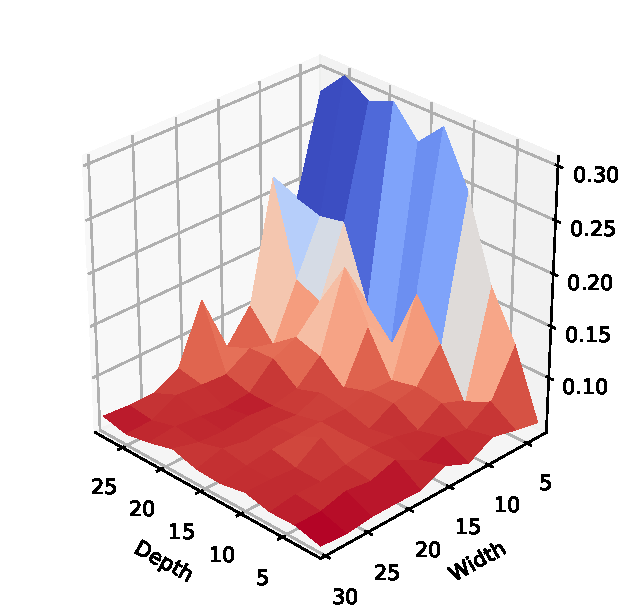
\includegraphics[width=\linewidth]{approach2-diff_yearly}
		\caption{}
	\end{subfigure}
	\begin{subfigure}{0.49\linewidth}
		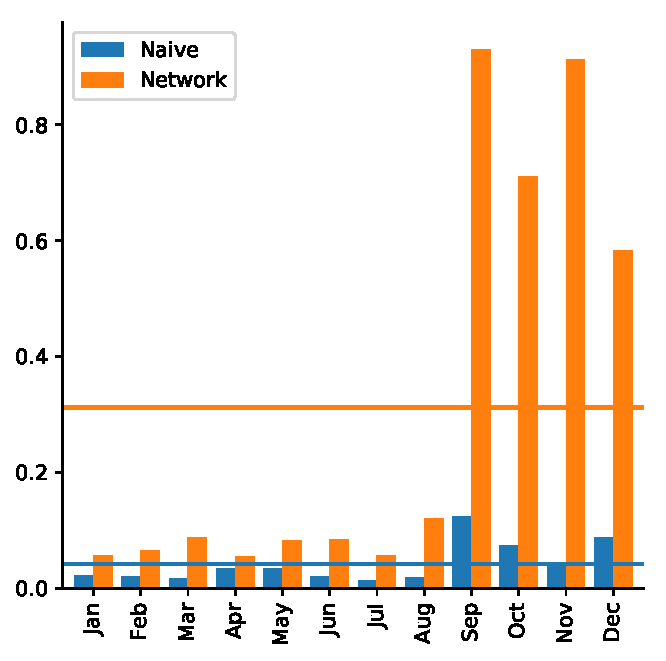
\includegraphics[width=\linewidth]{approach2-naive-comparison}
		\caption{}
	\end{subfigure}
	\caption[Evaluation using data in monthly representation]{Evaluation of network's performance using data in monthly representation. (a) Mean performance with respect to network width and depth. (b) Comparison of network with depth $L=1$ and width $K=30$ to naive prediction on the test set. The horizontal lines visualize the corresponding mean.}
	\label{fig:approach2-ex1}
\end{figure}

The results are shown in figure~\ref{fig:approach2-ex1}. While searching for an optimal combination of network depth and width (a) there are three findings:

\begin{enumerate}
	\item In contrast to the first approach it seams viable to increase the depth. Even with larger depth the loss seems acceptable. Furthermore there seems to be a correlation between loss and width because decreasing the width while at the same time increasing the depth stabilizes the loss.
	\item Nevertheless, the optimal combination is again depth $L=1$ and width $K=30$, albeit by a smaller margin.
	\item By comparing the predictions to a naive prediction -- assuming the spread prices are the same on the next day -- the results are disastrous. While the naive prediction is quite good with a mean of $0.04$ over all months the predictions are much worse with a mean of $0.31$. But also doing a monthwise comparison the performance of the network is always worse.
	The large difference in error between validation and test set also implies bad generalization properties.
\end{enumerate}

Even though during training the loss seemed acceptable, by validating the results on the test set the performance took a huge drop. In conclusion, the approach of using a monthly representation failed.

\subsection{Term structure representation's network}

Again, for each of the six legs of a spread prices' term structure a model with $L \in \{1,\dots,28\}$ and width $K \in \{3,\dots, 30\}$ is trained. This is repeated five times for each configuration for additional evaluation of variance. Therefore a total of $10 \cdot 10 \cdot 6 \cdot 5 = 3000$ models were trained. By first selecting the epoch with minimal validation loss per model, followed by taking the mean, one gets to evaluate depth and width as presented in figure~\ref{fig:approach2-ex2}.

\begin{figure}
	\centering
	\begin{subfigure}{0.49\linewidth}
		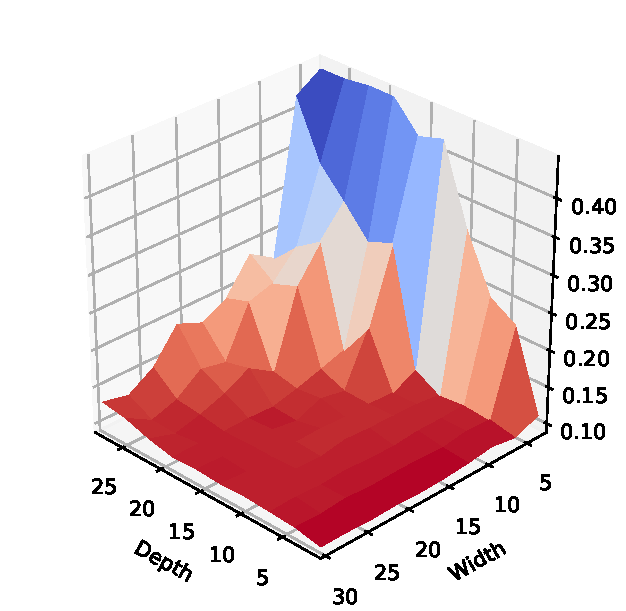
\includegraphics[width=\linewidth]{approach2-legwise}
		\caption{}
	\end{subfigure}
	\begin{subfigure}{0.49\linewidth}
		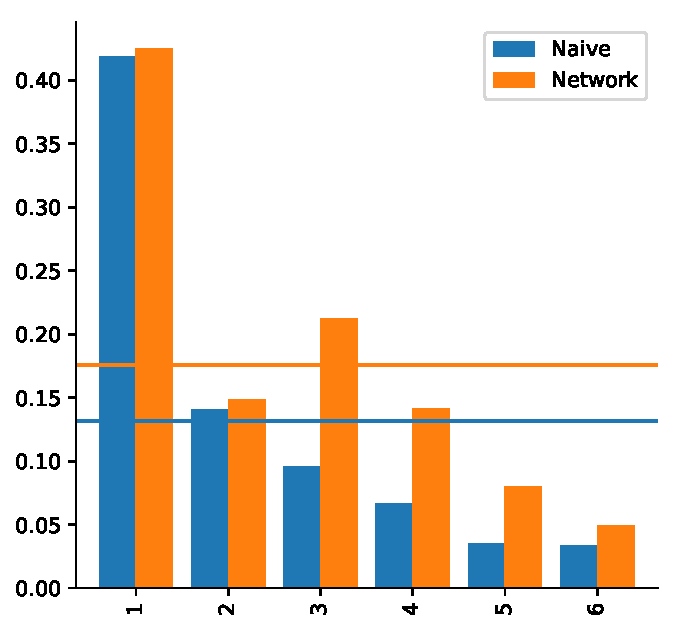
\includegraphics[width=\linewidth]{approach2-ex2-naive-comparison}
		\caption{}
	\end{subfigure}
	\caption[Evaluation using data represented as legs of a term structure]{Evaluation using data represented as legs of a term structure. (a) Mean performance with respect to network width and depth. (b) Comparison of network with depth $L=1$ and width $K=30$ to naive prediction on the test set. The horizontal lines visualize the corresponding mean.}
	\label{fig:approach2-ex2}
\end{figure}

The results are nearly identical to the former experiment using a monthly data representation. Most notably is the much smaller difference between the error values when comparing the networks' prediction (mean: $0.18$) and the naive prediction (mean: $0.13$). Nevertheless, beating the naive prediction did not work out, hence this approach is a failure, too.

By ordering the six networks' outputs, therefore forming a full term structure of tomorrows predicted spread prices, it is possible to make a comparison to the approach from chapter~\ref{ch:all-at-once}. Here, the resulting error is $0.176$ on the test set. Comparing this value to just the basic network from table~\ref{tab:aao-comparison} with error $0.156$ leads to the realization of the shortcomings of this approach. Dividing the work between several disconnected networks seems like a simplification, but at the end it just leads to similar or worse results. A possible cause might be the loss of context during optimization, where other outputs are not considered even if they possess a similar structure.

 
